\documentclass{article}

\usepackage{fullpage}
\usepackage{graphicx}
\usepackage{color}
\usepackage{url}

%
\usepackage{xspace}
\xspaceaddexceptions{(}
\newcommand{\GOAL}{\textsc{Goal}\xspace}

\definecolor{mygray}{gray}{0.75}
\makeatletter\newenvironment{graybox}
	{\begin{center}\begin{lrbox}{\@tempboxa}\begin{minipage}[t]{0.9\textwidth}}
	{\end{minipage}\end{lrbox}\colorbox{mygray}{\usebox{\@tempboxa}}\end{center}}
\makeatother


% DOCUMENT MANAGEMENT
\newcommand{\todo}[1]{\textbf{[TODO: }#1\textbf{]}}

%
%
\begin{document}

%
%
%
\title{The Game of Tic-Tac-Toe}
\author{Koen V. Hindriks}
\maketitle

%
%
%
\section{Introduction}
%
The game of Tic-Tac-Toe, also known as Noughts (Os) and crosses (Xs), is a game between two players, the X player and the O player.

%
%
%
\section{Playing Tic-Tac-Toe: An Example Agent Player}
%
\GOAL is distributed with one example agent player for the Tic-Tac-Toe game. This agent and its corresponding MAS file can be found in the \texttt{TicTacToe}
folder within the \texttt{GOALagents} folder that is located in the directory where \GOAL has been installed. If you did not start the IDE of \GOAL yet, do so now, and locate and load the MAS file \texttt{tictactoe.mas2g}. Select the MAS file and launch it by pressing the run button in the IDE of \GOAL. The game board depicted in Figure \ref{fig:gameBoard} should now be displayed.

\begin{figure}[h!]
\centering
    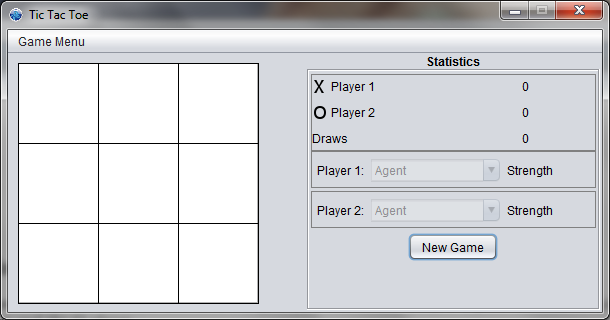
\includegraphics[width=0.75\textwidth]{gameBoard}
  \caption{The Tic-Tac-Toe Game Board}\label{fig:gameBoard}
\end{figure}


%
%
\subsection{Human Play}
%
If a player is a human, that player can interact with the game board using the mouse. The player options in the GUI of the game board can be used to select that a player is a human player. Indicating that a player is human can also be done by means of the initialization parameters in a MAS file (See Section \ref{sec:initialization}). Occupying a position on the board is as simple as clicking on that position.

Note that you can also start the game in a ``stand alone" mode and you do not need to start the IDE of \GOAL to play a game; see Section \ref{sec:environmentPackage}.


%
%
%
\section{Actions and Percepts in the Tic-Tac-Toe Game}\label{sec:ActionsAndPercepts}
%
The Tic-Tac-Toe game only supports the action to occupy a position on the game board. The occupy action can be performed if the position on the board has not yet been occupied in a previous move and it is the player's turn. A position occupied by a player is marked with that player's symbol, i.e., an `X' for the X player and an `O' for the O player.

\begin{graybox}
\texttt{occupy(Position)}: The argument \texttt{Position} can be \texttt{1}-\texttt{9}. The positions \texttt{1}, \texttt{3}, \texttt{7}, and \texttt{9} denote corners. Position \texttt{5} denotes the center of the game board.
\end{graybox}

The game board configuration is fully observable during the game. This means that both players can see exactly which positions have and have not yet been occupied and, if a position has been occupied, who has occupied it. For each of the nine positions on the board the following percept is received each round:

\begin{graybox}
\texttt{pos(Position, Player)}: The \texttt{Position} argument corresponds to one of the \texttt{1}-\texttt{9} positions. The player refers to the \texttt{x} or \texttt{o} player.
\end{graybox}

At the end of the game an agent player also receives information about who won the game.

\begin{graybox}
\begin{itemize}
	\item \texttt{winner(Player)}: The \texttt{Player} argument indicates who has won, either the \texttt{x} or \texttt{o} player. This percept only is received if there was a winner at the end of the game.
	\item \texttt{draw}: This percept is received at the end of the game if there was no winner.
\end{itemize}
\end{graybox}




%
%
%
\section{Environment Package Description}\label{sec:environmentPackage}
%

We briefly summarize here some relevant information about the environment:
\begin{description}
	\item[Name] The environment file is named \texttt{tictactoe.jar} and can be found in the \texttt{environments} folder that is located in the directory where \GOAL has been installed.
	\item[Pause] The environment supports pausing.
	\item[Reset] The environment supports reset.
	\item[Stand Alone] The environment supports stand alone running of a Tic-Tac-Toe game. \todo{How?}
\end{description}

%
%
\subsection{Initialization}\label{sec:initialization}
%

A game can be initialized by providing the types of players that will be playing the game. A player can be a human player, an agent player, or an AI player. A human player can play the game by using the game board and selecting a position the player wants to occupy by clicking on it with a mouse pointer. An agent player can occupy a position by performing the occupy action (see Section \ref{sec:ActionsAndPercepts}) and see the game board via percepts it receives from the game. An AI player is part of the environment itself. \todo{can we set strenght of AI player?}


The following initialization parameters can be set in the \texttt{environment} section of a MAS file:
\begin{graybox}
\begin{itemize}
	\item \texttt{xplayer}: can be set to values \texttt{"agent"}, \texttt{"ai"}, \texttt{"human"}. Selects the type of X player. See also explanation above. \textit{Example}: \texttt{xplayer = "agent"}.
	\item \texttt{oplayer}: can be set to values \texttt{"agent"}, \texttt{"ai"}, \texttt{"human"}. Selects the type of O player. See also explanation above. \textit{Example}: \texttt{oplayer = "human"}.
	\item \texttt{gui}: can be set to \texttt{"true"} or \texttt{"false"}. If set to true, the game board is displayed; otherwise it is not. \textit{Example}: \texttt{gui = "false"}.
\end{itemize}
\end{graybox}
 


\end{document}
